\documentclass{article}
\usepackage{epsfig}
\usepackage{graphicx}
\usepackage[top=0.50in, bottom=0.50in, left=0.65in, right=0.75in]{geometry}
%\usepackage[a4paper, total={6in, 10in}]{geometry}
\usepackage[table]{xcolor}
\usepackage{tikz}
\usepackage{algorithm}
\usepackage{mathtools}
\usepackage{amsmath,amssymb}
\usepackage[]{algpseudocode}
\usepackage{enumitem}
\title{CS345 Theoretical Assignment 1 \\ }
\author{\vspace{2mm} \large Ayush Agarwal, 13180 \\ M.Arunothia, 13378}
\date{}
\begin{document}
\maketitle
\tableofcontents
\newpage
\section{Neister Tree}
\subsection{Overview}
Given a complete graph G(E,V), we construct neister tree of set X by using nodes in $\{G \backslash X\}$ in a brute force manner.
Neister tree on X is a set Z so that $X \subset Z \subset V$, together with a spanning tree T of G[Z] such that weight of MST(G[Z]) is minimum.

\subsection{Maximum value of $Z$ }
\textbf{Lemma 1}: Any node n $\in$ $\{Z \backslash X\}$ will have $\textbf{degree}>=3$ in MST(G[Z]).\\
\textbf{Proof}: 
\begin{itemize} \itemsep -3pt
\item \textbf{degree}(n) can't be 0 since it $\in$ MST(G[Z]) which is fully connected.
\item \textbf{degree}(n) can't be 1 because a Spanning Tree can be constructed by just dropping n, whose weight will be less than MST(G[Z]). In that case Z won't be neister tree.
\item Suppose node n $\in$ {Z\\X} is connected to only 2 nodes (say x and y) in M=MST(G[Z]).
 Using Triangle Inequality we can say that,\\
 \hspace*{1cm}  $\boldsymbol{\omega}(n,x) $+$ \boldsymbol{\omega}(n,y) >= \boldsymbol{\omega}(x,y)$ \\ 
 Now, we can have a Spanning Tree $S$ in which there is an edge between x and y, and n is absent.\\
 \hspace*{1cm} \textbf{weight}(S)$= \textbf{weight}(M) - \boldsymbol{\omega}(n,x) - \boldsymbol{\omega}(n,y) + \boldsymbol{\omega}(x,y) <= \textbf{weight}(M)$\\
 Contradiction.  
\end{itemize}
Hence we can say that $\textbf{degree}(n)>=3$ in MST(G[Z]).\\
\\
Lets calculate the maximum value of $Z$. Suppose $\mid Z\backslash X\mid = p$.\\
In a tree, $\sum_V \textbf{degree}(v) = 2E$. In case of MST(G[Z]), minimum degree of p and k vertices are 3 and 1 respectively. \\
\hspace*{1cm} $\implies 3p + k <= 2(p+k-1)$     \hspace*{1cm}$\because E=V-1$ in a tree\\
\hspace*{1cm} $\implies p<=k-2$\\

\subsection{Pseudo-Code}
\begin{itemize} \itemsep -3pt
        \item \textbf{n} $= \mid V\mid$ 
        \item \textbf{vertexSet(G, k)}: returns a set of k distinct vertices from G which is different from previously returned sets
        \item \textbf{min\_weight}: holds the minimum weight of all the trees seen so far.
        \item \textbf{neisterTree}: Holds the set of vertices(Z) which can be potential Neister-Tree.    
\end{itemize}
\begin{algorithmic}[1]
\Procedure{NeisterTree($G, X, V$)}{}
\State min\_weight $\gets$ \textbf{MST}(G[X])
\State neisterTree $\gets$ X
\State $T \gets \{G\backslash X\}$
\For{$i$ in 0 \textbf{to} $k-2$}
\For{$j$ in 1 \textbf{to} $^{n-k} C_i$}
\State $Z \gets X\cup \textbf{vertexSet}(T,i)$ 
\State $temp \gets \textbf{MST}(G[Z])$
\If{temp $\leq$ min\_weight}
\State min\_weight $\gets$ temp
\State neisterTree $\gets$ Z
\EndIf
\EndFor
\EndFor
\State return neisterTree
\EndProcedure
\end{algorithmic}

\subsection{Time Complexity}
For every $i^{th}$ iteration, time req. is \\
\hspace*{1cm}$^{n-k} C_i *\textbf{MST(Z)}  <=$  $^{n-k} C_i * n^2$\\
Summing up time for every iteration,\\
\hspace*{1.2cm} $^{n-k} C_0 * n^2 + ^{n-k} C_1 * n^2 + ^{n-k} C_2 * n^2 + ... +  ^{n-k} C_{k-1} * n^2 + ^{n-k} C_k * n^2$\\
\hspace*{1cm} $=$ $ ^{n-k+1} C_{k+1} * n^2 $\\
\hspace*{1cm} $\leq$ $^{n} C_{k+1} * n^2 $\\
\hspace*{1cm} $\leq$ $n^{k+1}  * n^2 $\\
\hspace*{1cm} $\leq$ $n^{\mathcal{O}(k)}$\\
\hspace*{1cm} So time Complexity is $\boldsymbol{\mathcal{O}(n^{\mathcal{O}(k)})}$\\

\subsection{Justification}
This algorithm uses brute force to cover all cases. Basically it iterates over every possible subset of $\{V\backslash X\}$ of cardinality less than k-1, calculating the weight of the MST thus formed and takes minimum of them. The tree with the minimum weight is our answer.\\  

\newpage
\section{Unique-path graph}
\subsection{Overview}
Given there exists a vertex $u$ which has a path to every other vertex, we approach by first finding out vertex $u$. Now, we apply a single DFS from $u$ and keep extra tracker of $Back\_edge\_to$ to check for unique-path nature of the graph.
\subsection{Algorithm}
\begin{itemize}
\item Start
\item Mark all vertices unvisited. 
\item Start DFS from every vertex that is unvisited and mark them visited whenever they get visited in the process. Also estimate start and finish times of every vertex.
\item Let $u$ = Vertex with maximum finish time.
\item Start a DFS from vertex $u$. Exit with false if any cross edge, forward edge, or more than one back edge from any sub-tree is encountered as in these cases the graph cannot be unique-path graph.
\item Exit with true.
\item Stop.  
\end{itemize}
\subsection{Pseudo Code}
Run a DFS and find the vertex $v$ with maximum Finish Time. Now Run the following starting from $v$. 
\begin{algorithmic}[1]
\Procedure{DFS($v$)}{}
\State UniquePathGraph $\gets$ true
\State \textbf{Visited}[v] $\gets$ true
\State D[v] $\gets$ $count++$
\State \textbf{backEdge[v]} $\gets$ Null
\For{each edge $(v,w)$}
\If{ \textbf{Visited}[v] $=$ false}
\State $DFS(w)$;
\State t $\gets$ backEdge[w]
\If{t$<>$ Null \&\& Finished[t]$=$false \&\& t$<>$v }
\State backEdge[v] = t
\EndIf
\ElsIf{\textbf{Finished}[w]}
\State UniquePathGraph $\gets$ false
\State break;
\ElsIf{\textbf{backEdge[v]} $=$ Null}
\State \textbf{backEdge[v]} $\gets$ $w$
\Else
\State UniquePathGraph $\gets$ false
\State break;
\EndIf
\EndFor
\State \textbf{Finished}[w] $\gets$ true;
\State F[v] $\gets$ $count++$
\EndProcedure
\end{algorithmic}

\subsection{Time Complexity : }
\begin{itemize}
\item Locating the vertex $u$ takes a single DFS for every unvisited vertex - O(m+n)
\item From $u$ we make a single DFS - O(m+n)
\item Therefore, overall it is O(m+n) algorithm.
\end{itemize}

\subsection{Proof of Correctness}
\textbf{Lemma 1:} DFS from a vertex v visits all the unvisited vertices which are reachable from v.
\textbf{Proof:} Follows from the lemma discussed in the class. 

\newpage
\section{A real life application of Directed Acyclic Graphs}
\subsection{Overview}
This problem is approached by exploiting the topological ordering of DAGs. By the definition of root and exit, they will appear on the leftmost and rightmost ends of the ordering.
\subsection{Algorithm}
\begin{itemize}
\item Start.
\item Sort the vertices to get their topological ordering. Let $path$ be an array, defined as - $path[i]$ stores the number of distinct paths from root to the $i^{th}$ node in the topological ordering. Initialize all entries of this array with $0$. and $path[0] = 1$
\item Let $i=1$, $node_1$ denotes the first vertex after root in order. Run the following step till $i <> n-1$
\item For all incoming vertices to this $i^{th}$ node : edge ($node_j, node_i$) exists
\begin{itemize}
\item assign edge weight as $path[i]$
\item $path[i] += path[j]$
\end{itemize} 
\item Stop.
\end{itemize}
\subsection{Pseudo Code}
Assign\_edge\_weight(V,E)	\\*
\{			\\*
	\hspace*{1cm}node[ ] = topological\_sort(V,E) \\*
	\hspace*{1cm}path[ ] = $0$ \\*
	\hspace*{1cm}path[0] = $1$ \\*
	\hspace*{1cm} $i = node[1]$ // $node[0$] will be $root$\\*
	\hspace*{1cm} while$(i <> n-1)$  \\*
	\hspace*{2cm} For all $(node[j], node[i]) \in E$ \\*
	\hspace*{3cm} $w(node[j], node[i]) = path[i]$ \\*
	\hspace*{3cm} $path[i] += path[j]$ \\*
	\hspace*{1cm}return \\*
\}
\subsection{Time Complexity}
\begin{itemize}
\item Topological sorting - single DFS (using Finish Time) $= O(m+n)$
\item O(while\_loop) = O(sum of in degrees in the graph) $= O(m+n)$
\item Hence, overall time for a query is $O(m+n)$. 
\end{itemize}
\subsection{Proof of Correctness}
\subsubsection{What is to be proved? or Claim}
After $i$ iterations, $node j \in \{1,2,..,i\}$ will have $path[j]$ to be the number of distinct paths that start from the root and end in $node[j]$. Each of these paths will be assigned a unique path id between $0$ and $path[j]-1$.  
\subsubsection{Proof by Induction}
Induction is carried out on the iterator $i$
\subsubsection{Base Cases}
\begin{itemize}
\item $(i=1)$ - Only one edge from root to this $node_1$. 
\item $w(root,node_1) = path[1] = 0$  
\item $path[1] = path[0] + 0 = 1$
\item Hence, claim satisfies base case.
\item Notice, if there was no edge from root also, the claim will still hold.
\end{itemize}
\subsubsection{Hypothesis}
Let us assume that the Claim is true for all $i<=k$ where $k>1$ and both are integers.
\subsubsection{Inductive Step}
Let us prove that claim for $ k+1 $ is true.
\begin{center}
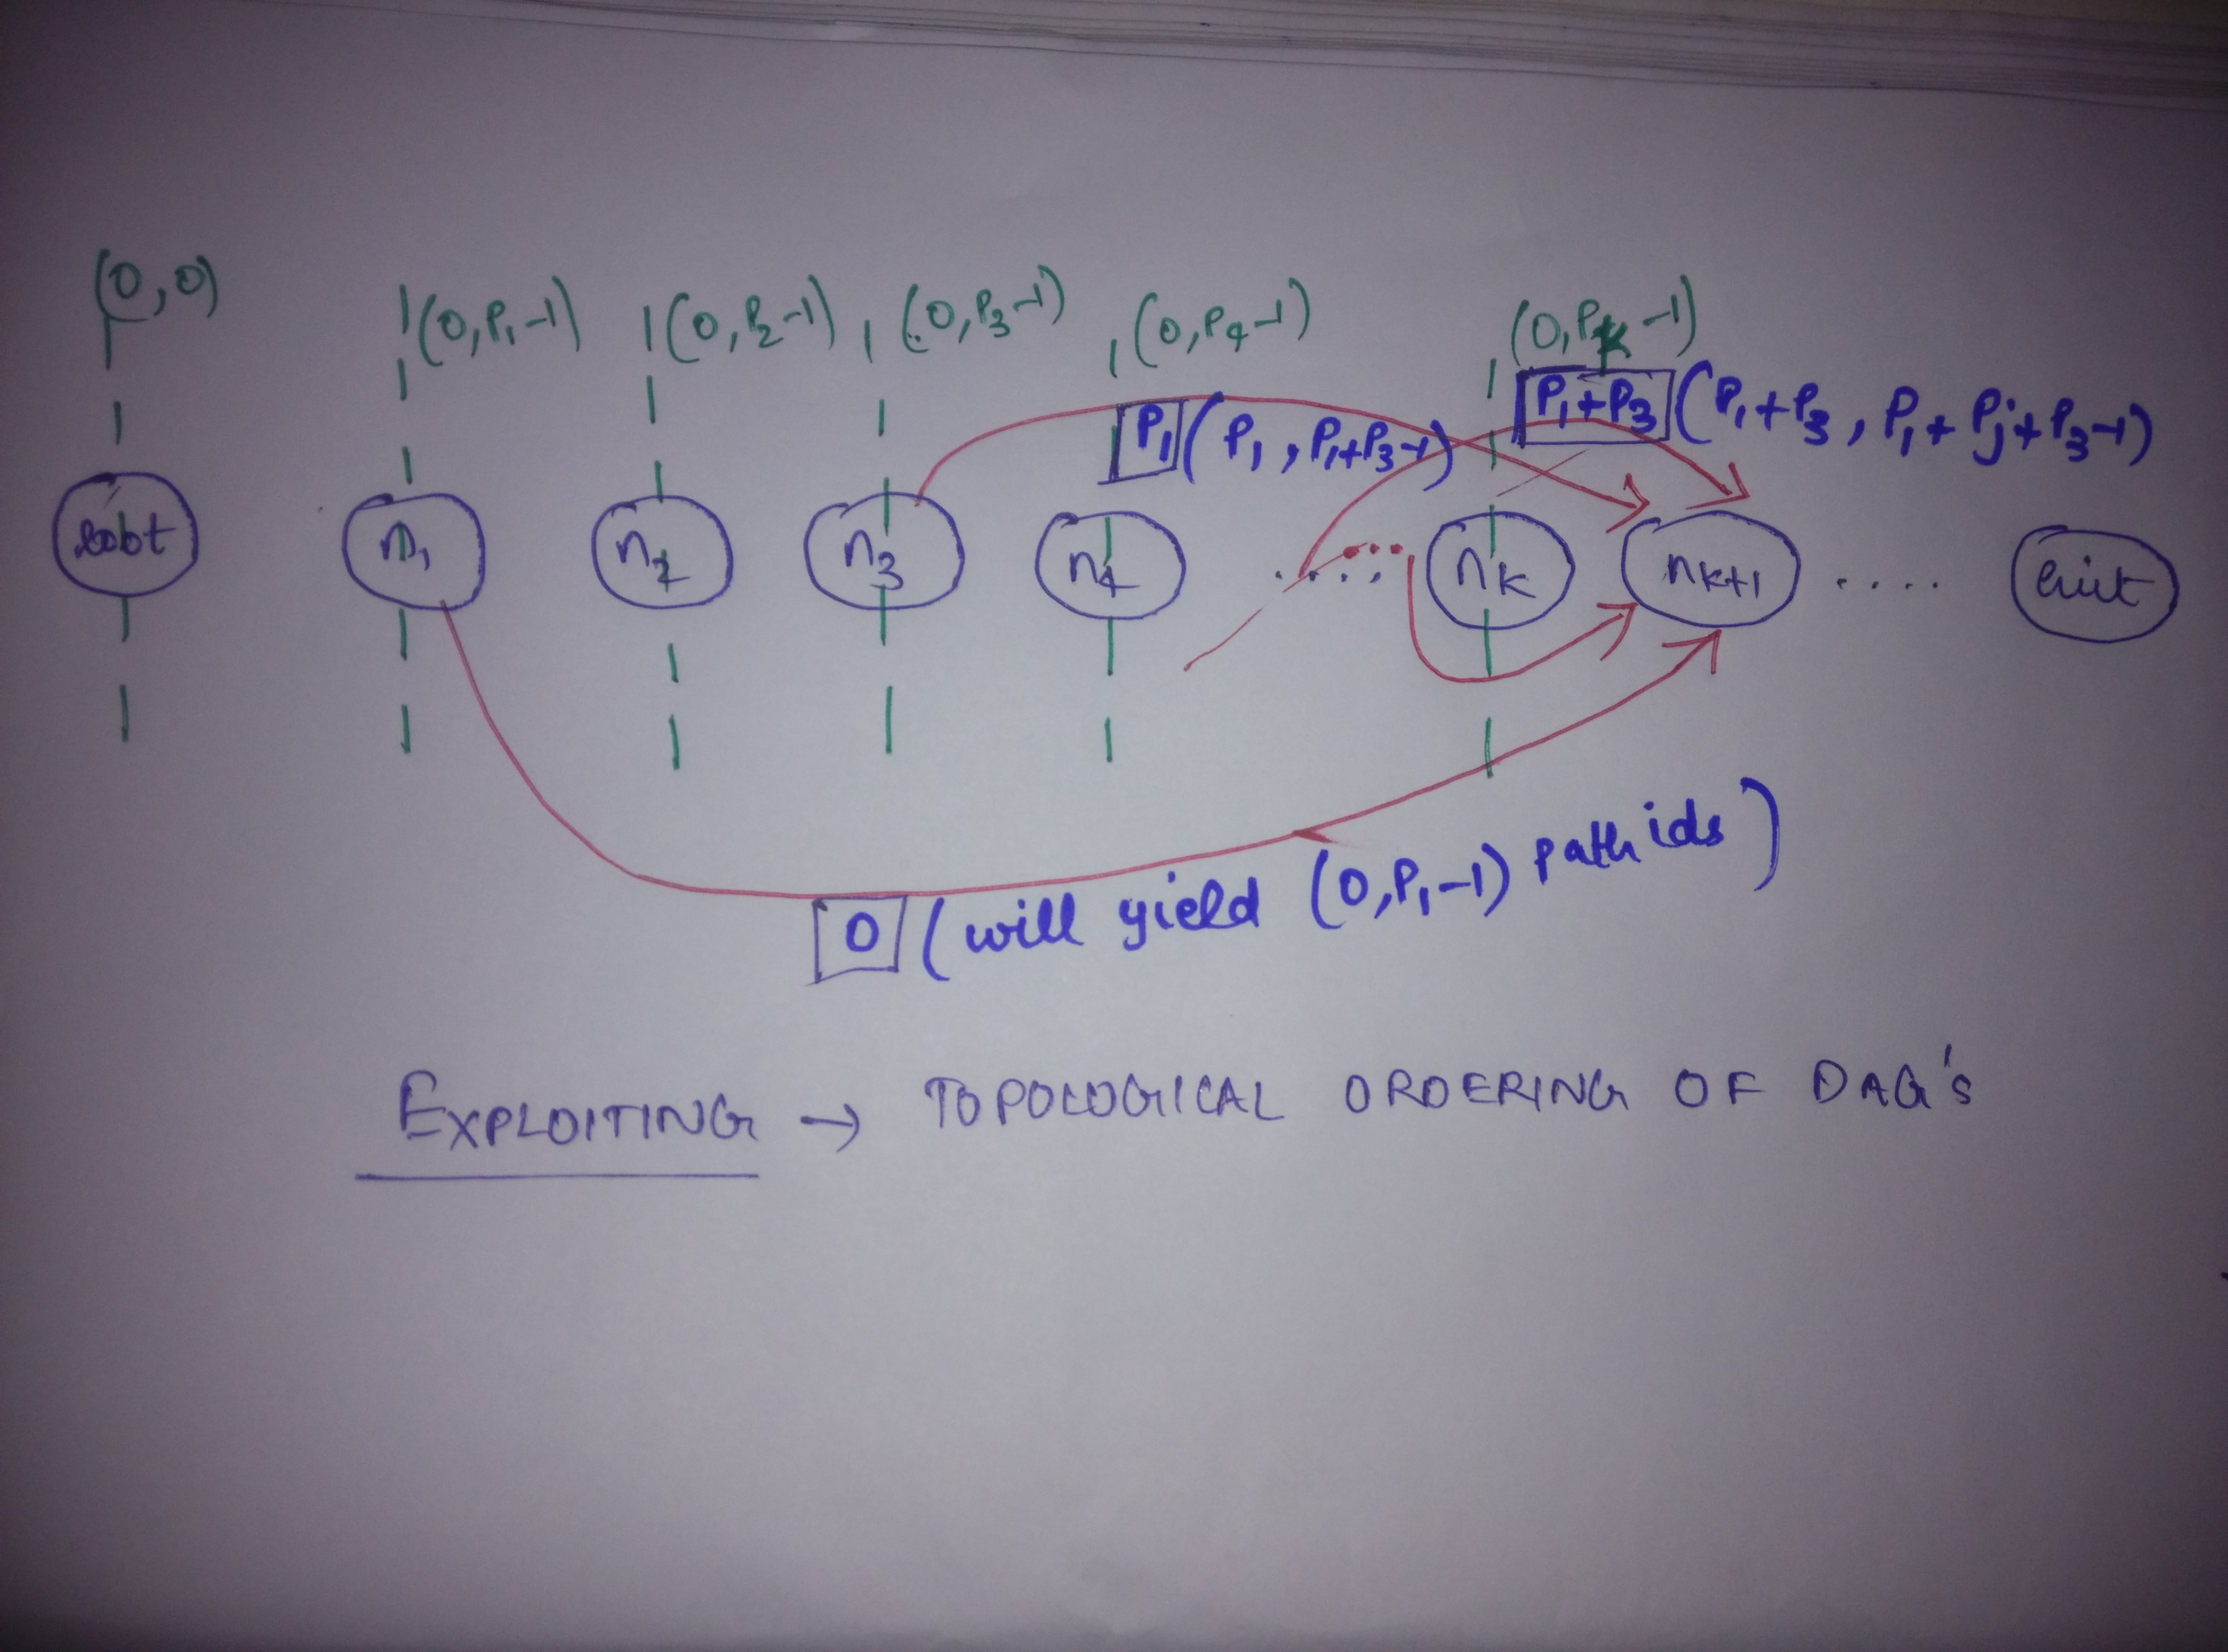
\includegraphics[scale=0.09]{3.jpg}
\end{center}
\begin{itemize}
\item if $(node_j, node_{k+1}) \in E$ then $j<k+1$ as they are in topological order. 
\item From inductive hypothesis we know 
\begin{itemize}
\item $path[j]$ - The total number of distinct paths from root to $node_j$.
\item Every path from $root$ to $node_j$ have unique path-ids $\in [0,path[j]-1]$.
\end{itemize}
\item $w(node_j, node_{k+1}) = path[k+1]$ will help maintain distinct path-ids as the paths that were encountered to reach $node_{k+1}$ would have been assigned path-ids between $0$ and $path[k+1]-1$. This new set of paths to $node_{k+1}$ via $node_{j}$ will get path-ids in $(path[k+1], path[k+1] +path[j])$.
\item Notice that every such $j$ will add $path[j]$ number of distinct paths to reach $node_{k+1}$ from the root. Hence, $path[k+1] += path[j]$ updates that in the loop.
\item Hence, the claim holds for $k+1$.
\item Thus, proved by induction.
\end{itemize}
\end{document}
